% fig_5_1_contributions_overview -- TikZ source of thesis Figure 19 (fig:contributions_overview).
% Every label is taken from the text of thesis Chapters 4-6; Gap B status: "Addressed, not closed".
% Layout (KTU thesis guide, section 5.1: figure text >= 10 pt): node-sized cards; all text at
% 10 pt (normalsize of the 10 pt standalone), panel headings and the centre title 12 pt bold.
% Panel heights follow the card contents.
% Natural width 15.44 cm: include at width=\textwidth (15.5 cm text block), scale ~1.
\documentclass[border=1pt]{standalone}
\usepackage[T1]{fontenc}
\usepackage{newtxtext,newtxmath}
\usepackage{amsmath}
\usepackage{tikz}
\usetikzlibrary{positioning,calc,backgrounds}

% Print-safe pale panel fills (luminance ~92-94%), dark borders/badges (luminance ~33-36%), black text.
\definecolor{cFill}{RGB}{232,243,230}\definecolor{cEdge}{RGB}{60,110,60}    % contributions
\definecolor{gFill}{RGB}{229,238,248}\definecolor{gEdge}{RGB}{50,90,140}    % gaps
\definecolor{lFill}{RGB}{251,239,216}\definecolor{lEdge}{RGB}{130,85,15}   % limitations
\definecolor{sFill}{RGB}{239,233,246}\definecolor{sEdge}{RGB}{100,70,135}   % strands
\definecolor{hub}{RGB}{45,45,45}

\begin{document}
\hyphenpenalty=10000 \exhyphenpenalty=10000
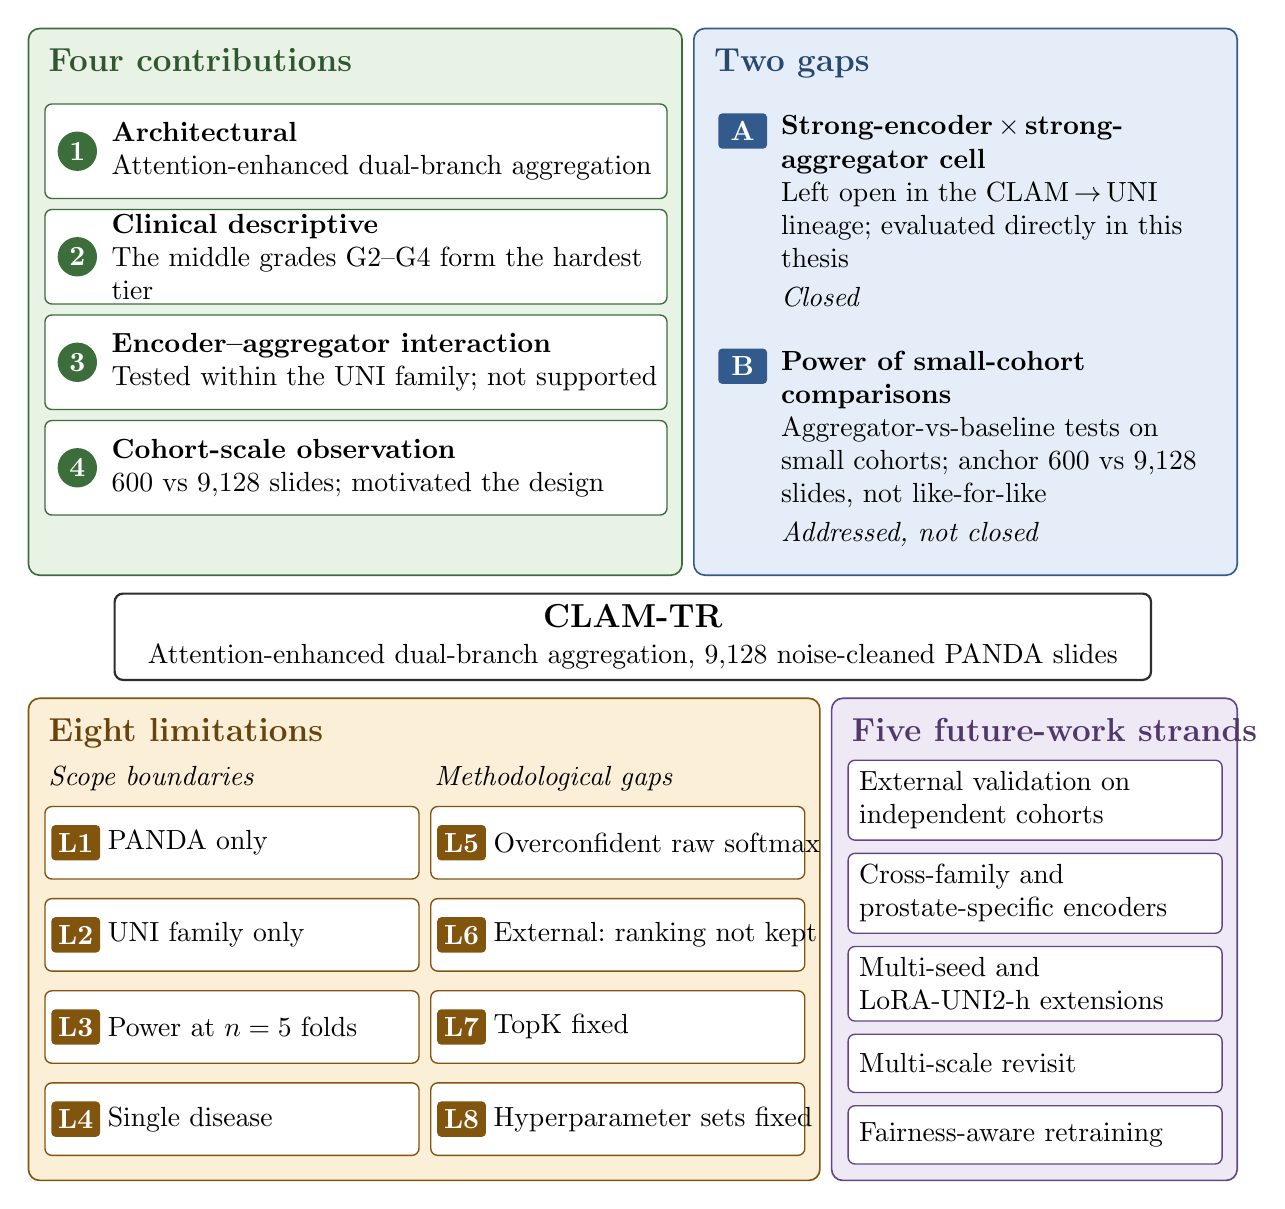
\begin{tikzpicture}[x=1cm, y=1cm, font=\normalsize,
    panel/.style={rounded corners=4pt, line width=0.6pt},
    card/.style={draw, rounded corners=2.5pt, line width=0.5pt, fill=white, align=flush left,
                 inner xsep=4pt, inner ysep=4pt},
    txt/.style={align=flush left, inner sep=0pt},
    head/.style={font=\large\bfseries, anchor=north west, inner sep=0pt},
    sub/.style={font=\itshape, anchor=north west, inner sep=0pt},
    badge/.style={circle, inner sep=0pt, minimum size=0.50cm, font=\bfseries, text=white},
    tag/.style={rounded corners=1.5pt, inner sep=0pt, minimum height=0.45cm, minimum width=0.62cm,
                font=\bfseries, text=white}]

  % geometry (cm): total width 15.35
  %   top row:    contributions panel 0-8.30 (cards 0.20-8.10); gaps panel 8.45-15.35 (cards 8.65-15.15)
  %   centre:     CLAM-TR card centred at 7.675
  %   bottom row: limitations panel 0-10.05 (two card columns 0.20-4.95, 5.10-9.85);
  %               strands panel 10.20-15.35 (cards 10.40-15.15)
  \coordinate (xR) at (15.35,0);  \coordinate (xM) at (7.675,0);
  \coordinate (xC) at (8.30,0);   \coordinate (xG) at (8.45,0);
  \coordinate (xGa) at (8.65,0);  \coordinate (xGb) at (15.15,0);  \coordinate (xGt) at (9.07,0);
  \coordinate (xL) at (10.05,0);  \coordinate (xS) at (10.20,0);   \coordinate (xSc) at (10.40,0);
  \coordinate (x0) at (0,0);

  % ======================= top-left: four contributions =======================
  \node[head, text=cEdge!80!black] (hC) at (0.25,-0.25) {Four contributions};
  \foreach \i/\ttl/\dsc in {%
      1/Architectural/Attention-enhanced dual-branch aggregation,
      2/Clinical descriptive/The middle grades G2--G4 form the hardest tier,
      3/Encoder--aggregator interaction/Tested within the UNI family; not supported,
      4/Cohort-scale observation/{600 vs 9,128 slides; motivated the design}}{%
    \pgfmathsetmacro{\yt}{-0.95-1.34*(\i-1)}
    \node[card, draw=cEdge, anchor=north west, minimum width=7.90cm, minimum height=1.20cm] (c\i) at (0.20,\yt) {};
    \node[txt, anchor=west, text width=6.95cm] at ([xshift=0.85cm]c\i.west) {\textbf{\ttl}\\\dsc};
    \node[badge, fill=cEdge] at ([xshift=0.42cm]c\i.west) {\i};
  }

  % ======================= top-right: two gaps =======================
  \node[head, text=gEdge!80!black] (hG) at (8.70,-0.25) {Two gaps};
  % G1
  \node[txt, anchor=north west, text width=5.45cm] (g1t) at (9.55,-1.10) {%
    \textbf{Strong-encoder\,$\times$\,strong-aggregator cell}\\
    Left open in the CLAM\,$\rightarrow$\,UNI lineage; evaluated directly in this thesis\\[2pt]
    \textit{Closed}};
  % G2
  \node[txt, anchor=north west, text width=5.45cm] (g2t) at ([yshift=-0.55cm]g1t.south west) {%
    \textbf{Power of small-cohort comparisons}\\
    Aggregator-vs-baseline tests on small cohorts; anchor 600 vs 9,128 slides, not like-for-like\\[2pt]
    \textit{Addressed, not closed}};
  \begin{scope}[on background layer]
    \draw[card, draw=gEdge] ($(xGa |- g1t.north)+(0,0.15)$) rectangle ($(xGb |- g1t.south)+(0,-0.15)$);
    \draw[card, draw=gEdge] ($(xGa |- g2t.north)+(0,0.15)$) rectangle ($(xGb |- g2t.south)+(0,-0.15)$);
  \end{scope}
  \node[tag, fill=gEdge, anchor=north] at ($(xGt |- g1t.north)+(0,0.03)$) {A};
  \node[tag, fill=gEdge, anchor=north] at ($(xGt |- g2t.north)+(0,0.03)$) {B};

  % ======================= top-row panels (equal height) =======================
  \path let \p1=(c4.south), \p2=(g2t.south) in coordinate (topbot) at (0,{min(\y1,\y2-0.15cm)-0.20cm});
  \begin{scope}[on background layer]
    \filldraw[panel, fill=cFill, draw=cEdge] (0,0) rectangle (xC |- topbot);
    \filldraw[panel, fill=gFill, draw=gEdge] (xG)  rectangle (xR |- topbot);
  \end{scope}

  % ======================= centre card =======================
  \node[draw=hub, fill=white, rounded corners=3pt, line width=0.8pt, align=flush center,
        inner xsep=12pt, inner ysep=4pt, anchor=north] (hubcard) at ($(xM |- topbot)+(0,-0.22)$) {%
    {\large\bfseries CLAM-TR}\\[1pt]
    Attention-enhanced dual-branch aggregation, 9,128 noise-cleaned PANDA slides};

  % ======================= bottom-left: eight limitations =======================
  \coordinate (btop) at ($(x0 |- hubcard.south)+(0,-0.22)$);
  \node[head, text=lEdge!80!black] (hL) at ($(btop)+(0.25,-0.25)$) {Eight limitations};
  \node[sub] (sL1) at ($(hL.south west)+(0,-0.22)$) {Scope boundaries};
  \node[sub] (sL2) at ($(hL.south west)+(4.90,-0.22)$) {Methodological gaps};
  \foreach \c/\r/\lab/\txt in {%
      0/1/L1/PANDA only, 0/2/L2/UNI family only, 0/3/L3/Power at $n = 5$ folds, 0/4/L4/Single disease,
      1/1/L5/Overconfident raw softmax, 1/2/L6/External:\ ranking not kept,
      1/3/L7/TopK fixed, 1/4/L8/Hyperparameter sets fixed}{%
    \pgfmathsetmacro{\xl}{0.20+4.90*\c}
    \coordinate (xl) at (\xl,0);
    \path ($(sL1.south)+(0,{-0.18-1.17*(\r-1)})$) coordinate (yy);
    \node[card, draw=lEdge, anchor=north west, minimum width=4.75cm, minimum height=0.92cm] (l\c\r) at (xl |- yy) {};
    \node[tag, fill=lEdge] at ([xshift=0.40cm]l\c\r.west) {\lab};
    \node[txt, anchor=west] at ([xshift=0.80cm]l\c\r.west) {\txt};
  }

  % ======================= bottom-right: five future-work strands =======================
  \node[head, text=sEdge!80!black] (hS) at ($(btop)+(10.45,-0.25)$) {Five future-work strands};
  \foreach \r/\txt in {%
      1/External validation on independent cohorts,
      2/Cross-family and prostate-specific encoders,
      3/Multi-seed and LoRA-UNI2-h extensions,
      4/Multi-scale revisit,
      5/Fairness-aware retraining}{%
    \ifnum\r=1 \path ($(hS.south)+(0,-0.22)$) coordinate (yy);
    \else \pgfmathtruncatemacro{\rp}{\r-1}\path ($(s\rp.south)+(0,-0.15)$) coordinate (yy); \fi
    \node[card, draw=sEdge, anchor=north west, minimum width=4.75cm, minimum height=0.74cm,
          text width=4.75cm-8pt] (s\r) at (xSc |- yy) {\txt};
  }

  % ======================= bottom-row panels (equal height) =======================
  \path let \p1=(l14.south), \p2=(s5.south) in coordinate (botbot) at (0,{min(\y1,\y2)-0.20cm});
  \begin{scope}[on background layer]
    \filldraw[panel, fill=lFill, draw=lEdge] (btop)        rectangle (xL |- botbot);
    \filldraw[panel, fill=sFill, draw=sEdge] (xS |- btop)  rectangle (xR |- botbot);
  \end{scope}
\end{tikzpicture}
\end{document}
